\begin{center}
	\section{数据结构}
\end{center}

\begin{multicols*}{2}

	\subsection{单调栈}

	求右边第一个大于自己的数的下标，没有则记 $0$。

	\begin{minted}{cpp}
deque<ll> q;
FOR(i, 1, N) {
    while (q.empty() == false
           && A[i] > A[q.back()]) {
        Ans[q.back()] = i;
        q.pop_back();
    }
    q.push_back(i);
}
FOR(i, 1, N) cout << Ans[i] << " ";
cout << "\n";
	\end{minted}

	\textbf{什么时候能用单调栈？}求解条件和单调条件\textbf{一致}（或至少有关联，比如相反）即可。例如已知一组上界 \texttt{up[i]}（满足 \texttt{up[i] < A[i]}），想为每个 $i$ 找最近的 $j > i$ 使得 \texttt{up[j] - j >= -i + A[i]}：可以让单调栈维护 $-j + A_j$ 的单调性，把比 \texttt{up[i] - i} 大的那些 $-j + A_j$ 都弹掉——因为 \texttt{up[j] < A[j]}，所以 \texttt{up[j] - j >= -i + A[i]} 时 \texttt{A[j] - j >= -i + A[i]} 也成立。

	\begin{minted}{cpp}
q.clear();
FOR(i, 1, N) {
    // 维护 -j + A[j] 的单调性
    while (q.empty() == false
           && up[i] - i < -q.back() + A[q.back()]) {
        seb[q.back()] = i;
        q.pop_back();
    }
    q.push_back(i);
}
	\end{minted}

	\subsection{离散化}

	将值域很大但数量有限的数据映射到连续的小区间上，常用于线段树、树状数组等需要以值作为下标的场景。

	\textbf{使用方法}：

	\begin{enumerate}
		\item 创建对象并用 \texttt{add} 添加所有需要离散化的值，然后调用 \texttt{init()} 完成排序去重。
		\item \texttt{get\_i(x)}：返回 $x$ 在离散化后的新下标。
		\item \texttt{operator[](idx)}：根据新下标反查原始值。
		\item \texttt{projectLr(l, r)}：将原始区间 $[l, r]$ 投影到离散化空间，返回新区间 $[li, ri]$ 以及是否合法。
		\item \texttt{contains(x)}：查询 $x$ 是否在离散化集合中。
		\item 通过 \texttt{shift} 控制下标基准（$0$ 为 0-based，$1$ 为 1-based）。
	\end{enumerate}

	\href{https://github.com/hh2048/XCPC/blob/484e9e0e6e4f127f187eb3df5bc419e9ec863795/02\%20-\%20\%E6\%89\%93\%E5\%8D\%B0\%E7\%A8\%BF\%E6\%A8\%A1\%E6\%9D\%BF\%E6\%B1\%87\%E6\%80\%BB/08\%20-\%20\%E6\%95\%B0\%E6\%8D\%AE\%E7\%BB\%93\%E6\%9E\%84.md\#L737}{参考来源：hh2048/XCPC 数据结构模板}

	\begin{minted}{cpp}
/* 参考了 hh2048/XCPC
 * AC https://acm.hdu.edu.cn/contest/view-code?cid=1200&rid=14607
 * 上面这个测试了这个 projectLr,get_i 应该是没什么问题
 */
 template<typename T>
struct Compress_ {
	// shift=0 就是采用 0-based 下标
	// shift=1 就是采用 1-based 下标
	int n, shift = 0;
	vector<T> liLs;

	Compress_() {
	}

	// 预估大小
	Compress_(ll n_) {
		liLs.reserve(n_);
	}

	Compress_(vector<T> in) : liLs(in) {
		init();
	}

	void add(T x) {
		liLs.emplace_back(x);
	}

	template<typename... Args>
	void add(T x, Args... args) {
		add(x), add(args...);
	}

	void init() {
		liLs.emplace_back(numeric_limits<T>::max());
		sort(liLs.begin(), liLs.end());
		liLs.resize(unique(liLs.begin(), liLs.end()) - liLs.begin());
		this->n = liLs.size();
	}

	int size() {
		return n;
	}

	int get_i(T x) {
		// 返回 x 元素的新下标
		return lower_bound(liLs.begin(), liLs.end(), x) - liLs.begin() + shift;
	}

	struct ProjectResult {
		bool ok;
		int l, r;
	};

	ProjectResult projectLr(T l, T r) {
		// 将区间 [l, r] 投影到离散化空间
		// li: 第一个 >= l 的离散化位置
		// ri: 最后一个 <= r 的离散化位置
		int li = (int) (lower_bound(liLs.begin(), liLs.end(), l) - liLs.begin()) + shift;
		int ri = (int) (upper_bound(liLs.begin(), liLs.end(), r) - liLs.begin()) - 1 + shift;
		return {li <= ri, li, ri};
	}

	T operator[](int idx) {
		// 根据新下标返回原来元素
		assert(idx - shift < n);
		return idx - shift < n ? liLs[idx - shift] : -1;
	}

	bool contains(T x) {
		// 查找元素 x 是否存在
		return binary_search(liLs.begin(), liLs.end(), x);
	}

	void reserve(ll n_) {
		liLs.reserve(n_);
	}

	friend auto &operator<<(ostream &o, const auto &j) {
		cout << "{";
		for (auto it: j.alls) {
			o << it << " ";
		}
		return o << "}";
	}
};
	\end{minted}

	典型用法示例：

	\begin{minted}{cpp}
Compress_<int> compress;
// 添加需要离散化的值
compress.add(100, 200, 500);
compress.init();

// 查询离散化后的下标
int idx = compress.get_i(200); // 1 (0-based)

// 反查原始值
int val = compress[1]; // 200

// 区间投影
auto [ok, l, r] = compress.projectLr(100, 500);
// ok=true, l=0, r=2
	\end{minted}

	\subsection{ST 表（Sparse Table）}

	ST 表用于 $O(n \log n)$ 预处理、$O(1)$ 回答静态区间\textbf{可重复贡献查询}（如区间最值、区间 GCD 等）。模板通过模板参数 \texttt{F} 接受任意二元运算，支持函数对象和 lambda。

	\begin{minted}{cpp}
/*
 * AC https://codeforces.com/contest/2175/submission/352780861
 * 实现了 op 函数的传入（可传入 lambda）
 * AC https://codeforces.com/contest/2205/submission/365029208
 */
template<class T, class F>
struct ST {
	ll N;
	vector<vector<T> > dp;
	F op;

	ST(ll N, const vector<T> &a, F fun)
		: N(N), dp(__lg(N) + 1,
			vector<T>(N + 5)), op(fun) {
		for (int i = 1; i <= N; ++i) {
			dp[0][i] = a[i];
		}
		for (int lay = 1; lay <= __lg(N); ++lay) {
			for (int i = 1;
				i <= N - (1 << (lay - 1)); ++i) {
				dp[lay][i] = op(dp[lay - 1][i],
					dp[lay - 1][i + (1 << (lay - 1))]);
			}
		}
	}

	T query(ll l, ll r) {
		ll lay = __lg(r - l + 1);
		return op(dp[lay][l],
			dp[lay][r - (1 << lay) + 1]);
	}
};
	\end{minted}

	\textbf{定长数组版（全局定义，防爆栈）}

	上面的 \texttt{vector} 版每次构造都要动态分配；下面这版把 \texttt{dp} 换成定长二维数组、运算用\textbf{函数指针模板参数} \texttt{T (*op)(T, T)}（编译期确定，可内联，零开销），必须\textbf{全局或 static 定义}，否则栈上放不下。\texttt{init} 只要求 \texttt{a[i]} 可下标访问，\texttt{vector} / 裸数组 / 指针都能传。

	\begin{minted}{cpp}
/* 2026/8/1 定长数组版, 全局定义防爆栈
 * MAXN 传最大下标即可 (内部已 +5)
 * 下标 1..N, 闭区间 query(l, r)
 * 用法: const int N = 200005;
 *   int mx(int a, int b) { return max(a, b); }
 *   ST<int, mx, N> st;   <- 必须全局 / static
 *   st.init(n, a);       <- a 是 vector 或 int a[N]
 */
template<class T, T (*op)(T, T), int MAXN>
struct ST {
private:
	static constexpr int LOG = __lg(MAXN) + 1;
	ll N;
	T dp[LOG][MAXN + 5];

public:
	ST() {}

	template<class A>
	ST(ll N, const A &a) { init(N, a); }

	// a 只需支持 a[i], i 取 1..n
	// vector / T[] / T* / array 均可
	template<class A>
	void init(ll n, const A &a) {
		N = n;
		for (int i = 1; i <= N; ++i) {
			dp[0][i] = a[i];
		}
		for (int lay = 1; lay <= __lg(N); ++lay) {
			for (int i = 1;
				i + (1 << lay) - 1 <= N; ++i) {
				dp[lay][i] = op(dp[lay - 1][i],
					dp[lay - 1][i + (1 << (lay - 1))]);
			}
		}
	}

	T query(ll l, ll r) {
		ll lay = __lg(r - l + 1);
		return op(dp[lay][l],
			dp[lay][r - (1 << lay) + 1]);
	}
};
	\end{minted}

	\subsection{树状数组（BIT / Fenwick Tree）}

	按支持的「修改方式 + 查询方式」分成三个版本，从简单到复杂依次是：单点加区间和、区间加单点查、区间加区间和。所有版本下标都从 $1$ 开始，且都依赖 \verb|lowbit(x) = x & (-x)|。

	下图是 $n = 8$ 时 BIT 的经典结构示意图：第 $i$ 格的条形宽度就是 \verb|lowbit(i)|，最右那格（白色）标号为 $i$，下面标它的二进制。连线表示「合并关系」，即 \verb|tr[i]| 由哪几个更小的块拼出来。

	\begin{center}
		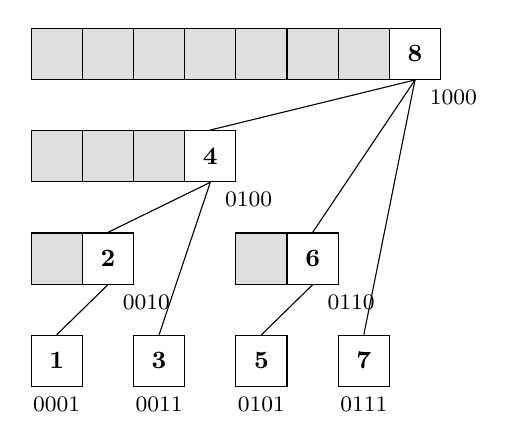
\begin{tikzpicture}[
			x=0.65cm, y=0.65cm,
			cell/.style={draw, minimum width=0.65cm, minimum height=0.65cm,
			inner sep=0pt, font=\small\bfseries},
			gcell/.style={cell, fill=gray!25},
			icell/.style={cell, fill=white},
			binl/.style={font=\footnotesize, inner sep=2pt}
		]
			% 各层 y 坐标
			\def\ya{0}
			\def\yb{2}
			\def\yc{4}
			\def\yd{6}

			% 底层（i 为奇数，lowbit = 1）
			\node[icell] (n1) at (1,\ya) {1};
			\node[icell] (n3) at (3,\ya) {3};
			\node[icell] (n5) at (5,\ya) {5};
			\node[icell] (n7) at (7,\ya) {7};
			\node[binl] at (1,\ya-0.85) {0001};
			\node[binl] at (3,\ya-0.85) {0011};
			\node[binl] at (5,\ya-0.85) {0101};
			\node[binl] at (7,\ya-0.85) {0111};

			% 第二层（lowbit = 2）
			\node[gcell]      at (1,\yb) {};
			\node[icell] (n2) at (2,\yb) {2};
			\node[gcell]      at (5,\yb) {};
			\node[icell] (n6) at (6,\yb) {6};
			\node[binl] at (2.75,\yb-0.85) {0010};
			\node[binl] at (6.75,\yb-0.85) {0110};

			% 第三层（lowbit = 4）
			\foreach \x in {1,2,3} \node[gcell] at (\x,\yc) {};
			\node[icell] (n4) at (4,\yc) {4};
			\node[binl] at (4.75,\yc-0.85) {0100};

			% 第四层（lowbit = 8）
			\foreach \x in {1,...,7} \node[gcell] at (\x,\yd) {};
			\node[icell] (n8) at (8,\yd) {8};
			\node[binl] at (8.75,\yd-0.85) {1000};

			% 管辖/合并关系
			\draw (n8.south) -- (n4.north);
			\draw (n8.south) -- (n6.north);
			\draw (n8.south) -- (n7.north);
			\draw (n4.south) -- (n2.north);
			\draw (n4.south) -- (n3.north);
			\draw (n2.south) -- (n1.north);
			\draw (n6.south) -- (n5.north);
		\end{tikzpicture}
	\end{center}

	例如 $\verb|tr[8]|$ 覆盖区间 $[1,8]$，它正好由 $\verb|tr[4]|$（管 $[1,4]$）、$\verb|tr[6]|$（管 $[5,6]$）、$\verb|tr[7]|$（管 $\{7\}$）和 $a_8$ 本身拼成；而 $\verb|tr[4]|$ 又由 $\verb|tr[2]|$、$\verb|tr[3]|$ 和 $a_4$ 拼成。所有 BIT 操作（\verb|add| 沿 \verb|i += lowbit(i)| 向上、\verb|query| 沿 \verb|i -= lowbit(i)| 向左跳）都能从这张图里直接读出来。

	\subsubsection{单点加，区间求和}

	最基础的 BIT：\verb|add(p, x)| 给位置 $p$ 加上 $x$，\verb|query(l, r)| 返回 \verb|a[l]+a[l+1]+...+a[r]|。下面这份在常规功能之外还带两个小工具，前提是数组里只存 $0/1$（常用于维护一个动态可重集的占位表）：

	\begin{itemize}
		\item \verb|findkth(k)|：从左往右数第 $k$ 个 $1$ 所在的位置。
		\item \verb|kthspace(k)|：从左往右数第 $k$ 个 $0$ 所在的位置。
	\end{itemize}

	两者思路一样：在 BIT 上按位倍增地往右走，每到一步判断「这个块里 $1$（或 $0$）的总数够不够吃掉剩下的 $k$」，够就跨过，不够就留在当前位置继续往下走。整个过程 $O(\log n)$。

	\begin{minted}{cpp}
// by znzryb
// 普通的单点修改区间查询树状数组，
// 含有查找第K个空位，第K个元素的功能
// https://www.codechef.com/viewsolution/1179893708
//   查找第K个元素测试
// 第K个空位的测试应该是一道abc的题目，但是当时没保存
struct BIT {
	vector<ll> tr;
	int n;

	inline int lowbit(int x) {
		return x & (-x);
	}

	BIT(int ln) {
		n = ln;
		tr.resize(n + 5, 0);
	}
	BIT() {}

	inline void add(int p, ll x) {
		if (p == 0) return;
		while (p <= n) {
			tr[p] += x;
			p += lowbit(p);
		}
	}

	inline ll query(int l, int r) {
		ll lres = 0, rres = 0;
		l -= 1;
		while (l > 0) {
			lres += tr[l];
			l -= lowbit(l);
		}
		while (r > 0) {
			rres += tr[r];
			r -= lowbit(r);
		}
		return rres - lres;
	}

	// 找到第 k 个元素，要求只能出现 0 和 1
	inline int findkth(int k) {
		int x = 0, sum = 0;
		for (int i = __lg(n); ~i; --i) {
			x += 1 << i;
			if (x >= n || sum + tr[x] >= k) {
				x -= 1 << i;
			} else {
				sum += tr[x];
			}
		}
		// 始终让 cx < k，+1 就是新元素出现的位置
		return x + 1;
	}

	// 找到第 k 个空位，要求只能出现 0 和 1
	inline int kthspace(int k) {
		int cx = 0;
		// 不断缩小步长的搜索
		for (int i = 1 << 20; i > 0; i >>= 1) {
			if (cx + i <= n &&
				lowbit(cx + i) - tr[cx + i] < k) {
				// lowbit(cx+i) - tr[cx+i]
				//   即该 BIT 块内的空位数
				k -= lowbit(cx + i) - tr[cx + i];
				cx += i;
			}
		}
		return cx + 1;
	}
};
	\end{minted}

	\subsubsection{区间加，单点查询}

	BIT 不再维护原数组 \verb|a|，而是维护差分数组 \verb|d[i] = a[i] - a[i-1]|。这样：

	\begin{itemize}
		\item \textbf{区间加} \verb|a[l..r] += x|：只改差分的两个位置，\verb|d[l] += x; d[r+1] -= x;|
		\item \textbf{单点查} \verb|a[p]|：就是差分的前缀和 \verb|d[1] + d[2] + ... + d[p]|，BIT 天然支持。
	\end{itemize}

	所以这一版的 \verb|add(l, r, x)| 就是对差分做两次单点加，\verb|query(p)| 就是差分的前缀和查询。

	\begin{minted}{cpp}
struct BIT {
	// 支持区间修改，单点查询（使用差分实现）
	// https://www.luogu.com.cn/record/221012815
	vector<ll> tr;
	int n;

	ll lowbit(ll x) {
		return x & (-x);
	}

	BIT(int n_) {
		n = n_;
		tr.resize(n, 0);
	}

	// 差分的单点加，内部用
	void add(ll p, ll x) {
		while (p <= n) {
			tr[p] += x;
			p += lowbit(p);
		}
	}

	// 区间加：a[l..r] += x
	//   等价于 d[l] += x, d[r+1] -= x
	void add(ll l, ll r, ll x) {
		r += 1;
		add(l, x);
		add(r, -x);
	}

	// 单点查 a[p] = d[1] + d[2] + ... + d[p]
	ll query(ll p) {
		ll ret = 0;
		while (p) {
			ret += tr[p];
			p -= lowbit(p);
		}
		return ret;
	}
};
	\end{minted}

	\subsubsection{区间加，区间求和}

	继续沿用差分 \verb|d[i] = a[i] - a[i-1]|。区间加依然是两次 \verb|d[l] += x; d[r+1] -= x|。难点在区间和查询，先看怎么算前缀和 \verb|a[1] + a[2] + ... + a[P]|，把每一项用差分展开：

	\begin{minted}{text}
a[1..P] = d[1]
        + d[1] + d[2]
        + d[1] + d[2] + d[3]
        + ...
        + d[1] + d[2] + ... + d[P]

数一下每个 d[i] 出现了几次：
  d[1] 出现 P 次
  d[2] 出现 P-1 次
  ...
  d[i] 出现 (P - i + 1) 次

所以合并起来：
a[1..P] = sum{ d[i] * (P - i + 1), i = 1..P }
        = (P+1) * sum(d[1..P])
            - sum(i * d[i], i = 1..P)
	\end{minted}

	右边两项都是普通的前缀和，各用一个 BIT 就行：\verb|tr1| 存 \verb|d[i]|，\verb|tr2| 存 \verb|i * d[i]|。于是 \verb|query(P) = (P+1) * sum(tr1, P) - sum(tr2, P)|，区间和就是 \verb|query(r) - query(l-1)|。

	区间加 \verb|[l, r] += x| 时，两个 BIT 要同步改：

	\begin{minted}{text}
对 tr1 （存 d[i]）：
  tr1 在 l   处 += x
  tr1 在 r+1 处 -= x

对 tr2 （存 i * d[i]）：
  i = l   时：d[l]   += x  =>  i*d[i] +=   l  * x
  i = r+1 时：d[r+1] -= x  =>  i*d[i] -= (r+1) * x
	\end{minted}

	注意乘的系数 \verb|l|、\verb|r+1| 在修改时就是已知常数，所以能直接塞进 \verb|tr2| 的单点加里。

	\begin{minted}{cpp}

/* 2026-04-19 luogu 线段树模板题
 * AC https://www.luogu.com.cn/record/274702532
 * 进一步添加了 public,private 规定了接口的可见性
 * 2026-04-19 增强了对 0 的鲁棒性
 * AC https://acm.hdu.edu.cn/contest/view-code?cid=1201&rid=9803
 */
 class BIT {
	// 支持区间修改，区间查询
	// 维护两个差分：d[i] 和 i*d[i]
	// 前缀和 sum(p) = (p+1)*sum(d[1..p])
	//              - sum(i*d[i], 1..p)
	vector<ll> tr1, tr2;
	int n;

	ll lowbit(ll x) {
		return x & (-x);
	}

public:
	BIT(int n_) {
		n = n_;
		// 这个 n+1 就够了，虽然涉及到这个差分
		tr1.assign(n + 2, 0);
		tr2.assign(n + 2, 0);
	}

private:
	void add(vector<ll> &tr, ll p, ll x) {
		// 防止 0 死循环
		if (p <= 0) return;
		while (p <= n) {
			tr[p] += x;
			p += lowbit(p);
		}
	}

	ll sum(vector<ll> &tr, ll p) {
		ll ret = 0;
		while (p) {
			ret += tr[p];
			p -= lowbit(p);
		}
		return ret;
	}

	// 单点加
	void add(ll p, ll x) {
		add(tr1, p, x);
		add(tr2, p, p * x);
	}

public:
	// 区间加，[l, r] 每个位置加 x
	void add(ll l, ll r, ll x) {
		add(tr1, l, x);
		add(tr1, r + 1, -x);
		add(tr2, l, l * x);
		add(tr2, r + 1, -(r + 1) * x);
	}

private:
	// 前缀和 a[1] + a[2] + ... + a[p]
	ll query(ll p) {
		return (p + 1) * sum(tr1, p) - sum(tr2, p);
	}

public:
	// 区间和 a[l] + ... + a[r]
	ll query(ll l, ll r) {
		return query(r) - query(l - 1);
	}
};
	\end{minted}

	\paragraph{技巧：提前结算避免树状数组清零}

	\href{https://acm.hdu.edu.cn/contest/problem?cid=1201&pid=1007}{从这道题目学到的技巧}

	树状数组不支持高效的区间清零（需要逐点撤销）。但如果我们知道某段区间 $[l, r]$ 上累积的值最终要\textbf{贡献给谁}，就可以在需要“清零”的时刻，先把 BIT 上 $[l, r]$ 的当前和查出来、结算到对应的答案里，然后\textbf{不做任何清零操作}。之后 BIT 上再产生的增量会叠加在旧值之上，但因为旧值已经被结算走了，所以只要在最终统计时再查一次并减去"已结算部分"，效果就等价于清零后重新累加。

	典型场景：维护若干组的区间贡献，当某段区间的归属从旧组切换到新组时：

	\begin{minted}{cpp}
// 将 [l, r] 的归属从 originV 切换到 val，不清零 BIT
ll add = tr->query(l, r);   // 查出 [l, r] 上的已有增量
anss[originV] += add;        // 旧归属结算
anss[val] -= add;            // 新归属预扣（之后查询时会连带查出这部分旧值）
	\end{minted}

	\subsubsection{单点改，区间最值查询（BIT 实现 RMQ）}

	和求和不同，$\min / \max$ 这类运算\textbf{只有结合律、没有逆运算}（即没有「区间减法」），所以不能像前缀和那样用 $\text{pre}(r) - \text{pre}(l-1)$ 直接拿到任意区间的结果。不过 BIT 的分块结构只依赖结合律就够用了：每个 \verb|tr[i]| 管辖 \verb|a[i - lowbit(i) + 1 .. i]| 这个区间的最值，因此整个骨架仍然可以复用，只是查询和更新都必须按块拼凑，复杂度从 $O(\log n)$ 退化到 $O(\log^2 n)$。相对于 ST 表的优势是\textbf{支持在线单点修改}。

	\textbf{查询} \verb|query(l, r)|：从右端 \verb|r| 往左跳，每次能吃掉一整个 BIT 块就吃（\verb|tr[r]|，跨度 \verb|lowbit(r)|），吃不动的那一格（即 \verb|r - lowbit(r) < l| 的时候）退化为单独看 \verb|a[r]|，然后 \verb|r--| 继续：

	\begin{minted}{text}
res = dummy
while r >= l:
    res = op(res, a[r])        // 单独处理 a[r]
    r -= 1
    while r - lowbit(r) >= l:   // 尽量用 BIT 块跳
        res = op(res, tr[r])
        r -= lowbit(r)
	\end{minted}

	\textbf{更新} \verb|upd(p, x)|：把 \verb|a[p]| 覆盖为 \verb|x| 之后，所有「管辖 \verb|p| 的 BIT 块」都要重算。这些块的下标就是

	\begin{minted}{text}
i = p,
    p + lowbit(p),
    p + lowbit(p) + lowbit(p + lowbit(p)),
    ...
	\end{minted}

	也就是外层循环 \verb|i += lowbit(i)| 依次枚举的那些位置。由于没有区间减法，无法从旧 \verb|tr[i]| 里扣掉旧 \verb|a[p]| 的贡献，所以只能\textbf{从头合并整块}。

	好在 BIT 的管辖区间有一个漂亮的自相似分解——它能切成若干长度是 $2$ 的幂、两两不相交的子段，而这些子段本身就是已有的更小的 \verb|tr|：

	\begin{minted}{text}
tr[i] 管辖 [i - lowbit(i) + 1 .. i]，长度 lowbit(i)
可拆成：
    tr[i - lowbit(i)/2]    长度 lowbit(i)/2   // 左半
    tr[i - lowbit(i)/4]    长度 lowbit(i)/4   // 再右半的一半
    ...
    tr[i - 2]              长度 2
    tr[i - 1]              长度 1
    a[i]                   长度 1             // 自己这一格

验证：1 + 1 + 2 + 4 + ... + lowbit(i)/2 = lowbit(i)
      刚好铺满管辖区间。
	\end{minted}

	所以重算就是：

	\begin{minted}{text}
tr[i] = op(a[i],
           tr[i - 1],
           tr[i - 2],
           tr[i - 4],
           ...,
           tr[i - lowbit(i)/2])
	\end{minted}

	对应代码里的内层循环——让 \verb|j| 从 $1$ 按 $2$ 的幂翻倍直到 \verb|lowbit(i)/2|。

% \textbf{为什么 \texttt{tr[i - j]} 直接用旧值就对？}  把所有用到的小块按「管辖区间是否含 \verb|p|」分成两类：
% \begin{itemize}
% 	\item 含 \verb|p| 的：它一定是本轮外层循环在更早的某次迭代里刚被重算过的——因为 \verb|i += lowbit(i)| 保证我们总是\textbf{先处理更小的 i}，而含 \verb|p| 的那个小块的下标一定小于当前 \verb|i|。
% 	\item 不含 \verb|p| 的：它的值自始至终没变，自然是最新的。
% \end{itemize}

% 两种情况下 \verb|tr[i - j]| 都已经是最新值。单次 \verb|upd| 的复杂度：外层 $O(\log n)$ 次、每次内层合并至多 $O(\log n)$ 个小块，总共 $O(\log^2 n)$。

	\begin{minted}{cpp}
// by Gospel_rock znzryb
// 参考了（抄了）OIwiki
// AC https://www.luogu.com.cn/record/228807838
//   （ST 表模版题，max 版本）
// AC https://www.luogu.com.cn/record/228809172
//   （打乱了插入顺序，同题）
// AC https://codeforces.com/contest/2184/submission/358028437
// 进行了现代化改造，更加符合现在我们的习惯
struct RMQ {
	const ll dummy = INF;
	ll n;
	vector<ll> tr;
	vector<ll> origin;

	inline ll lowbit(const ll &x) {
		return x & -x;
	}

private:
	ll op(const ll &a, const ll &b) {
		return min(a, b);
	}

public:
	RMQ(ll n) {
		this->n = n + 2;
		tr.resize(n + 5, INF);
		origin.resize(n + 5);
	}

	ll query(ll l, ll r) {
		ll res = dummy;
		while (r >= l) {
			res = op(origin[r], res);
			r--;
			for (; r - lowbit(r) >= l; r -= lowbit(r)) {
				res = op(res, tr[r]);
			}
		}
		return res;
	}

	// 注意：语义是「把位置 p 覆盖为 x」，不是增加
	void upd(ll p, ll x) {
		origin[p] = x;
		for (int i = p; i <= n; i += lowbit(i)) {
			tr[i] = origin[i];
			for (int j = 1; j < lowbit(i); j <<= 1) {
				tr[i] = op(tr[i], tr[i - j]);
			}
		}
	}
};
	\end{minted}

	\textbf{切换 \texttt{min}/\texttt{max}}：把 \verb|op| 改成 \verb|max|、同时把 \verb|dummy| 从 \verb|INF| 改成 \verb|-INF| 即可。如果要泛化成任意幂等运算（操作一次和操作十次结果一样如，\verb|gcd|、按位与/或等），需要选一个对该运算「吸收」的恒元作为 \verb|dummy|。

	\subsection{珂朵莉树（ODT / Chtholly Tree）}

	珂朵莉树用 \verb|std::map| 维护若干不相交的「颜色段」\verb|[l, r, val]|。核心思路：\textbf{每次区间赋值把覆盖到的所有旧段一次性合并删除}，再插入一段新段。在随机数据或有大量区间覆盖操作的题目中，段数期望 $O(n \log n)$，因此总复杂度可接受。

	两个核心操作：
	\begin{itemize}
		\item \verb|split(pos)|：把包含 \verb|pos| 的段在 \verb|pos| 处切开，保证 \verb|pos| 是某段的左端点。
		\item \verb|assign(la, ra, val)|：先 \verb|split| 两端，然后一次性抹掉 $[la, ra]$ 内所有旧段，插入新段。在抹掉每段时可顺带做任意聚合统计（如下方用 BIT 查区间权重和并累到 \verb|anss| 上）。
	\end{itemize}

	\begin{minted}{cpp}
	/*
	 * 2026-04-19 内部式的 ODT
	 * AC https://acm.hdu.edu.cn/contest/view-code?cid=1201&rid=9850
	 */
	struct RVal {
		ll r;
		ll val;
	};

	map<ll, RVal> mpODT;

	void split(ll pos) {
		if (mpODT.empty()) return;
		auto it = mpODT.upper_bound(pos);
		if (it == mpODT.begin()) return;
		it--;
		// pos 就是左端点         pos 不在区间内
		if (it->first == pos || it->second.r < pos) {
			return;
		}
		mpODT[pos] = {it->second.r, it->second.val};
		it->second.r = pos - 1;
	}

	void assign(ll la, ll ra, ll val) {
		split(la);
		split(ra + 1);
		auto it = mpODT.lower_bound(la);
#ifdef LOCAL
		assert(it->first==la);
#endif
		for (; it != mpODT.end();) {
			if (it->first > ra) {
				break;
			}
			ll originV = it->second.val;
			ll l = it->first, r = it->second.r;
			// 这里是做一些事情，比如说累加答案
			// ll add = tr->query(l, r);
			// anss[originV] += add;
			// anss[val] -= add;
			it = mpODT.erase(it);
		}
		mpODT[la] = {ra, val};
	}
	\end{minted}

	\subsection{带权可撤销并查集（判二分图）}

	带权可撤销并查集（队友的模版），可以用来判断图是否是二分图。\textbf{一般和线段树分治绑定}：分治进入子区间前 \verb|snapshot()|，离开时 \verb|rollback()| 回到该快照，省去为每个时间区间重建图的代价。\verb|val[x]| 维护 \verb|x| 到 \verb|fa[x]| 的边权异或值，\verb|find| 不做路径压缩（路径压缩与回滚不兼容），靠按秩合并保 $O(\log n)$ 单次。\verb|badCnt| 计数当前累计的「奇环」（合并时 \verb|valx ^ valy != w| 即一条奇环），\verb|isBipartiteGraph()| 即 \verb|badCnt == 0|。

	\begin{minted}{cpp}
class RollbackDSU
{
  struct Info
  {
    int x, y, oldSizeY, oldBadCnt, oldValX;
    bool isMerged;
  };

  int badCnt;
  vector<int> fa, sz, val;
  stack<Info> history;

public:
  RollbackDSU(int n) : badCnt(0), fa(n + 1), sz(n + 1, 1), val(n + 1, 0)
  {
    iota(fa.begin(), fa.end(), 0);
  }

  int snapshot()
  {
    return (int)history.size();
  }

  void rollback(int snapshot)
  {
    while ((int)history.size() > snapshot)
    {
      auto [x, y, oldSizeY, oldBadCnt, oldValX, isMerged] = history.top();
      history.pop();

      badCnt = oldBadCnt;

      if (!isMerged)
      {
        continue;
      }

      val[x] = oldValX;
      sz[y] = oldSizeY;
      fa[x] = x;
    }
  }

  pair<int, int> find(int x)
  {
    int cur = 0;

    while (fa[x] != x)
    {
      cur ^= val[x];
      x = fa[x];
    }

    return {x, cur};
  }

  bool merge(int x, int y, int w)
  {
    auto [fx, valx] = find(x);
    auto [fy, valy] = find(y);

    if (fx == fy)
    {
      history.push({0, 0, 0, badCnt, 0, false});

      if ((valx ^ valy) != w)
      {
        badCnt++;
      }

      return false;
    }

    if (sz[fx] > sz[fy])
    {
      swap(fx, fy);
      swap(valx, valy);
    }

    history.push({fx, fy, sz[fy], badCnt, val[fx], true});

    sz[fy] += sz[fx];
    val[fx] = valx ^ valy ^ w;
    fa[fx] = fy;

    return true;
  }

  bool isBipartiteGraph() const
  {
    return badCnt == 0;
  }
};
	\end{minted}

	\subsection{线段树分治}

	线段树分治模板（队友的模版），常和上面的可撤销带权并查集绑定，用来\textbf{离线处理「在时间轴上每条边只在区间 $[l, r]$ 内存在」类型的问题}。把每条边按其存活时间区间挂到线段树对应的若干 $O(\log q)$ 个节点上；DFS 整棵线段树，进入节点前依次 \verb|merge| 该节点上挂的所有边，离开节点前 \verb|rollback| 到进入时的 \verb|snapshot|，到叶子时即可拿到该时间点的并查集状态（如查二分图：\verb|isBipartiteGraph()|）。

	\begin{minted}{cpp}
struct SegmentTreeDivide {
  int q;
  vector<vector<pair<int, int>>> seg;

  SegmentTreeDivide() {}

  SegmentTreeDivide(int q) {
    init(q);
  }

  void init(int q_) {
    q = q_;
    seg.assign(4 * q + 5, {});
  }

  void add(int node, int l, int r, int ql, int qr, pair<int, int> edge) {
    if (ql <= l && r <= qr) {
      seg[node].push_back(edge);
      return;
    }

    int mid = (l + r) >> 1;

    if (ql <= mid) {
      add(node << 1, l, mid, ql, qr, edge);
    }

    if (qr > mid) {
      add(node << 1 | 1, mid + 1, r, ql, qr, edge);
    }
  }

  void add(int l, int r, pair<int, int> edge) {
    if (l > r) {
      return;
    }

    add(1, 1, q, l, r, edge);
  }
};
	\end{minted}

\end{multicols*}

	\subsection[\tochl{ACL \texttt{segtree}（单点修改）}]{ACL \texttt{segtree}（单点修改）}
			\subsection{\texttt{segtree}：单点改 + 区间查（非递归）}

		维护满足\textbf{结合律}的二元运算 \texttt{op} 与其\textbf{单位元} \texttt{e}（即幺半群 monoid）上的序列，支持单点赋值 $O(\log n)$、区间求积 $O(\log n)$、以及在线段树上二分 $O(\log n)$。

		\textbf{接口一览}（$n$ 为序列长度，下标 0-based）：

		\begin{itemize}
			\item \texttt{segtree<S, op, e> seg(n)}：长度 $n$，全部初始化为 \texttt{e()}。
			\item \texttt{segtree<S, op, e> seg(v)}：由 \texttt{vector<S> v} 建树，$O(n)$。
			\item \texttt{seg.set(p, x)}：令 $a_p \leftarrow x$。
			\item \texttt{seg.get(p)}：返回 $a_p$。
			\item \texttt{seg.prod(l, r)}：返回 $op(a_l, \dots, a_{r-1})$；$l = r$ 时返回 \texttt{e()}。
			\item \texttt{seg.all\_prod()}：返回全区间积，$O(1)$。
			\item \texttt{seg.max\_right(l, f)}：返回最大的 $r$，使 $f(op(a_l, \dots, a_{r-1}))$ 为真。要求 \texttt{f} 单调（真在前假在后）且 \texttt{f(e())} 为真。
			\item \texttt{seg.min\_left(r, f)}：返回最小的 $l$，使 $f(op(a_l, \dots, a_{r-1}))$ 为真。同样要求 \texttt{f} 单调且 \texttt{f(e())} 为真。
		\end{itemize}

		\textbf{三个易错点}：

		\begin{enumerate}
			\item \texttt{op} 与 \texttt{e} 必须是\textbf{自由函数}（或函数指针 / 无捕获 lambda 转成的函数指针），\textbf{不能}是带捕获的 lambda——它们是模板参数，编译期就要定死。
			\item \texttt{e()} 必须是真单位元：求最大值时用足够小的哨兵（如 \texttt{-4e18}）而非 $0$，否则负数序列查询结果错。
			\item \texttt{prod} 是 $[l, r)$ 左闭右开；从 1-based 闭区间 $[L, R]$ 换算过来是 \texttt{prod(L - 1, R)}。
		\end{enumerate}

		\textbf{示例一：区间最大值}（单点赋值 + 区间查最大，完整可提交骨架）

		\begin{minted}{cpp}
/* 题意: n 个数, q 次操作
 *   1 p v -> 把第 p 个数改成 v  (1-based)
 *   2 l r -> 输出 [l, r] 里的最大值 (闭区间)
 */
using S = ll;   // 每个结点存什么: 这里就是值本身

// op: 两段的答案怎么合并成一段的答案
// 必须满足结合律 —— max 满足:
//   max(max(a,b),c) == max(a,max(b,c))
S op_max(S a, S b) { return max(a, b); }

// e: op 的单位元, 要求 op(e(), x) == x 恒成立
// 所以取「不可能出现的极小值」当哨兵。
// 千万别写 0: 全是负数时查询会错答成 0
S e_max() { return -4e18; }

int main() {
    int n, q;
    cin >> n >> q;

    vector<S> a(n);            // 全程 0-based
    for (auto &x: a) cin >> x;

    // 用 vector 一次性建树是 O(n);
    // 先 segtree(n) 再逐个 set 是 O(n log n),
    // 能一次建好就不要循环 set
    segtree<S, op_max, e_max> seg(a);

    while (q--) {
        int t;
        cin >> t;
        if (t == 1) {          // 单点赋值
            int p;
            ll v;
            cin >> p >> v;
            seg.set(p - 1, v); // 题面 1-based, 减 1
        } else {               // 区间查最大
            int l, r;
            cin >> l >> r;
            // prod 是左闭右开 [l, r), 而题面给的
            // 是闭区间 [l, r] -> 写成 prod(l-1, r)
            cout << seg.prod(l - 1, r) << "\n";
        }
    }
}
		\end{minted}

		\textbf{示例二：区间和 + 线段树上二分}。求「从 $l$ 出发最长的前缀，使区间和不超过 $x$」——这是 \texttt{max\_right} 的典型用途，把「外层二分 + 内层查询」的 $O(\log^2 n)$ 压到 $O(\log n)$：

		\begin{minted}{cpp}
using S = ll;
// 求和版三件套: 加法结合, 单位元是 0
S op_sum(S a, S b) { return a + b; }
S e_sum() { return 0; }

int main() {
    int n;
    ll x;
    cin >> n >> x;
    vector<S> a(n);
    for (auto &v: a) cin >> v;
    segtree<S, op_sum, e_sum> seg(a);

    int l = 0;   // 从下标 l 出发

    // 谓词 f 可以是「带捕获的 lambda」——
    // 它是普通函数参数, 不是模板参数,
    // 这点跟 op / e 的限制不同。
    // 要求 f 单调: 真在前、假在后, 且 f(e()) 真。
    // 这里 sum <= x 单调的前提是元素非负
    // (有负数时前缀和会上下摆, 谓词不单调,
    //  max_right 的返回值就没有意义了)
    int r = seg.max_right(l, [&](S sum) {
        return sum <= x;
    });

    // r 是「最大的下标」, 使
    //   a[l] + a[l+1] + ... + a[r-1] <= x
    // 所以能取的元素个数 = r - l
    cout << r - l << "\n";

    // 对称接口: min_left(r, f) 从右往左找
    // 最小的 l 使 a[l..r-1] 满足 f
    int l2 = seg.min_left(n, [&](S sum) {
        return sum <= x;
    });
    cout << n - l2 << "\n";  // 后缀能取几个
}
		\end{minted}

		\textbf{模板本体}：

		\begin{minted}{cpp}
/* AtCoder Library v1.6 atcoder/segtree 自包含移植
 * 改动: 去 #ifndef 守卫与 namespace atcoder,
 *      去 std:: 前缀, internal_bit 的
 *      bit_ceil / countr_zero 内联成私有 static
 * 约定: 下标 0-based, 区间 [l, r) 左闭右开
 */
template<class S, S (*op)(S, S), S (*e)()>
struct segtree {
public:
    segtree() : segtree(0) {}

    explicit segtree(int n)
        : segtree(vector<S>(n, e())) {}

    explicit segtree(const vector<S> &v)
        : _n(int(v.size())) {
        size = (int) bit_ceil((unsigned) _n);
        log = countr_zero((unsigned) size);
        d = vector<S>(2 * size, e());
        for (int i = 0; i < _n; i++)
            d[size + i] = v[i];
        for (int i = size - 1; i >= 1; i--)
            update(i);
    }

    // a[p] = x
    void set(int p, S x) {
        assert(0 <= p && p < _n);
        p += size;
        d[p] = x;
        for (int i = 1; i <= log; i++)
            update(p >> i);
    }

    // 返回 a[p]
    S get(int p) const {
        assert(0 <= p && p < _n);
        return d[p + size];
    }

    // 返回 op(a[l], ..., a[r - 1])
    S prod(int l, int r) const {
        assert(0 <= l && l <= r && r <= _n);
        S sml = e(), smr = e();
        l += size, r += size;
        while (l < r) {
            if (l & 1) sml = op(sml, d[l++]);
            if (r & 1) smr = op(d[--r], smr);
            l >>= 1, r >>= 1;
        }
        return op(sml, smr);
    }

    S all_prod() const { return d[1]; }

    // 最大的 r 使 f(op(a[l..r-1])) 为真
    template<class F>
    int max_right(int l, F f) const {
        assert(0 <= l && l <= _n);
        assert(f(e()));
        if (l == _n) return _n;
        l += size;
        S sm = e();
        do {
            while (l % 2 == 0) l >>= 1;
            if (!f(op(sm, d[l]))) {
                while (l < size) {
                    l = 2 * l;
                    if (f(op(sm, d[l]))) {
                        sm = op(sm, d[l]);
                        l++;
                    }
                }
                return l - size;
            }
            sm = op(sm, d[l]);
            l++;
        } while ((l & -l) != l);
        return _n;
    }

    // 最小的 l 使 f(op(a[l..r-1])) 为真
    template<class F>
    int min_left(int r, F f) const {
        assert(0 <= r && r <= _n);
        assert(f(e()));
        if (r == 0) return 0;
        r += size;
        S sm = e();
        do {
            r--;
            while (r > 1 && (r % 2)) r >>= 1;
            if (!f(op(d[r], sm))) {
                while (r < size) {
                    r = 2 * r + 1;
                    if (f(op(d[r], sm))) {
                        sm = op(d[r], sm);
                        r--;
                    }
                }
                return r + 1 - size;
            }
            sm = op(d[r], sm);
        } while ((r & -r) != r);
        return 0;
    }

private:
    int _n, size, log;
    vector<S> d;

    // 原 atcoder::internal::bit_ceil
    static unsigned bit_ceil(unsigned n) {
        unsigned x = 1;
        while (x < n) x *= 2;
        return x;
    }

    // 原 atcoder::internal::countr_zero
    static int countr_zero(unsigned n) {
        return __builtin_ctz(n);
    }

    void update(int k) {
        d[k] = op(d[2 * k], d[2 * k + 1]);
    }
};
		\end{minted}

		\textbf{与本模板其它线段树的取舍}：ACL 版是非递归实现，常数小、代码短，但\textbf{只支持单点修改}；要区间修改（区间加 / 区间赋值）请用下一小节的 \texttt{lazy\_segtree}，或主板子数据结构章的递归式懒标记线段树。ACL 版另一个优势是 \texttt{max\_right} / \texttt{min\_left} 这对树上二分接口，主板子的线段树模板没有等价物。


	\subsection[\tochl{ACL \texttt{lazy\_segtree}（区间修改）}]{ACL \texttt{lazy\_segtree}（区间修改）}
			在 \texttt{segtree} 的幺半群 $(S,op,e)$ 上再定义作用幺半群 $(F,composition,id)$，即可支持区间修改、区间查询和树上二分，单次操作均为 $O(\log n)$。

		\textbf{五件套约束}：\texttt{op} 必须满足结合律；\texttt{e} 是其单位元；\texttt{mapping(f,x)} 表示把作用 $f$ 施加到 $x$；\texttt{composition(f,g)} 表示“先 $g$ 后 $f$”；\texttt{id} 是恒等作用。作用还必须满足对 \texttt{op} 的分配律。

		\textbf{最大的坑}：\texttt{mapping} 拿不到区间边界。凡是更新公式需要长度，都要把 \texttt{len} 存进 $S$，让它随 \texttt{op} 一起合并。

		\textbf{接口}：除 \texttt{segtree} 的 \texttt{set/get/prod/all\_prod/max\_right/min\_left} 外，新增 \texttt{apply(p,f)} 与闭区间 \texttt{apply(l,r,f)}。因为查询前可能需要下推标记，\texttt{get/prod} 与两个二分接口不再是 \texttt{const}。

		\subsubsection{模板本体}

		\begin{minted}{cpp}
/* ACL atcoder/lazysegtree 自包含移植 + 闭区间
 * lazy_segtree(n) 合法位置 0..n; 区间 [l, r] 左闭右闭
 * 1-based 只碰 1..n; 0-based 只碰 0..n-1
 * 从 vector 建树时 v[i] 对应位置 i, 长度由 vector 决定
 * 空区间写 r == l - 1, prod 返回 e(), apply 直接返回
 */
template<class S, S (*op)(S, S), S (*e)(),
         class F, S (*mapping)(F, S),
         F (*composition)(F, F), F (*id)()>
struct lazy_segtree {
public:
    lazy_segtree() : lazy_segtree(0) {}

    explicit lazy_segtree(int n)
        : lazy_segtree(vector<S>(n + 1, e())) {}

    explicit lazy_segtree(const vector<S> &v)
        : _n(int(v.size())) {
        size = (int) bit_ceil((unsigned) _n);
        log = countr_zero((unsigned) size);
        d = vector<S>(2 * size, e());
        lz = vector<F>(size, id());
        for (int i = 0; i < _n; i++)
            d[size + i] = v[i];
        for (int i = size - 1; i >= 1; i--)
            update(i);
    }

    void set(int p, S x) {
        assert(0 <= p && p < _n);
        p += size;
        for (int i = log; i >= 1; i--) push(p >> i);
        d[p] = x;
        for (int i = 1; i <= log; i++) update(p >> i);
    }

    S get(int p) {
        assert(0 <= p && p < _n);
        p += size;
        for (int i = log; i >= 1; i--) push(p >> i);
        return d[p];
    }

    S prod(int l, int r) {
        r++;
        assert(0 <= l && l <= r && r <= _n);
        if (l == r) return e();
        l += size, r += size;
        for (int i = log; i >= 1; i--) {
            if (((l >> i) << i) != l) push(l >> i);
            if (((r >> i) << i) != r)
                push((r - 1) >> i);
        }
        S sml = e(), smr = e();
        while (l < r) {
            if (l & 1) sml = op(sml, d[l++]);
            if (r & 1) smr = op(d[--r], smr);
            l >>= 1, r >>= 1;
        }
        return op(sml, smr);
    }

    S all_prod() { return d[1]; }

    void apply(int p, F f) {
        assert(0 <= p && p < _n);
        p += size;
        for (int i = log; i >= 1; i--) push(p >> i);
        d[p] = mapping(f, d[p]);
        for (int i = 1; i <= log; i++) update(p >> i);
    }

    void apply(int l, int r, F f) {
        r++;
        assert(0 <= l && l <= r && r <= _n);
        if (l == r) return;
        l += size, r += size;
        for (int i = log; i >= 1; i--) {
            if (((l >> i) << i) != l) push(l >> i);
            if (((r >> i) << i) != r)
                push((r - 1) >> i);
        }
        {
            int l2 = l, r2 = r;
            while (l < r) {
                if (l & 1) all_apply(l++, f);
                if (r & 1) all_apply(--r, f);
                l >>= 1, r >>= 1;
            }
            l = l2, r = r2;
        }
        for (int i = 1; i <= log; i++) {
            if (((l >> i) << i) != l) update(l >> i);
            if (((r >> i) << i) != r)
                update((r - 1) >> i);
        }
    }

    template<class G>
    int max_right(int l, G g) {
        assert(0 <= l && l <= _n);
        assert(g(e()));
        if (l == _n) return _n - 1;
        l += size;
        for (int i = log; i >= 1; i--) push(l >> i);
        S sm = e();
        do {
            while (l % 2 == 0) l >>= 1;
            if (!g(op(sm, d[l]))) {
                while (l < size) {
                    push(l);
                    l = 2 * l;
                    if (g(op(sm, d[l]))) {
                        sm = op(sm, d[l]);
                        l++;
                    }
                }
                return (l - size) - 1;
            }
            sm = op(sm, d[l]);
            l++;
        } while ((l & -l) != l);
        return _n - 1;
    }

    template<class G>
    int min_left(int r, G g) {
        r++;
        assert(0 <= r && r <= _n);
        assert(g(e()));
        if (r == 0) return 0;
        r += size;
        for (int i = log; i >= 1; i--)
            push((r - 1) >> i);
        S sm = e();
        do {
            r--;
            while (r > 1 && (r % 2)) r >>= 1;
            if (!g(op(d[r], sm))) {
                while (r < size) {
                    push(r);
                    r = 2 * r + 1;
                    if (g(op(d[r], sm))) {
                        sm = op(d[r], sm);
                        r--;
                    }
                }
                return r + 1 - size;
            }
            sm = op(d[r], sm);
        } while ((r & -r) != r);
        return 0;
    }

private:
    int _n, size, log;
    vector<S> d;
    vector<F> lz;

    static unsigned bit_ceil(unsigned n) {
        unsigned x = 1;
        while (x < n) x *= 2;
        return x;
    }

    static int countr_zero(unsigned n) {
        return __builtin_ctz(n);
    }

    void update(int k) {
        d[k] = op(d[2 * k], d[2 * k + 1]);
    }

    void all_apply(int k, F f) {
        d[k] = mapping(f, d[k]);
        if (k < size)
            lz[k] = composition(f, lz[k]);
    }

    void push(int k) {
        all_apply(2 * k, lz[k]);
        all_apply(2 * k + 1, lz[k]);
        lz[k] = id();
    }
};
		\end{minted}

		\begin{multicols*}{2}

			\subsubsection{示例：区间加 + 区间和}

			区间长度必须存进 $S$；空出来的 0 号位置长度为 $0$，因此不会影响 1-based 查询。

			\begin{minted}{cpp}
// ACL_EXAMPLE: lazy_range_add_sum
struct S {
    ll sum;
    int len;
};
using F = ll;

S op(S a, S b) {
    return {a.sum + b.sum, a.len + b.len};
}
S e() { return {0, 0}; }
S mapping(F f, S x) {
    return {x.sum + f * x.len, x.len};
}
F composition(F f, F g) { return f + g; }
F id() { return 0; }

using SegAddSum = lazy_segtree<S, op, e, F,
        mapping, composition, id>;

// vector<S> a(n + 1, e());
// FOR(i, 1, n) a[i] = {x[i], 1};
// SegAddSum seg(a);
// seg.apply(l, r, add);
// ll ans = seg.prod(l, r).sum;
			\end{minted}

			\subsubsection{示例：仿射修改 + 一至三次幂和}

			用 $x\leftarrow ax+b$ 统一表达乘法、加法与赋值：乘 $v$ 是 \texttt{\{v,0\}}，加 $v$ 是 \texttt{\{1,v\}}，赋值 $v$ 是 \texttt{\{0,v\}}。节点同时维护 $\sum x$、$\sum x^2$、$\sum x^3$。

			\begin{minted}{cpp}
// ACL_EXAMPLE: lazy_affine_moments
const ll MOD = 998244353;

ll mul_mod(ll a, ll b) {
    return (ll)((__int128)a * b % MOD);
}

struct S {
    ll s1, s2, s3;
    int len;
};
struct F {
    ll mul, add; // x <- mul * x + add
};

S op(S x, S y) {
    return {(x.s1 + y.s1) % MOD,
            (x.s2 + y.s2) % MOD,
            (x.s3 + y.s3) % MOD,
            x.len + y.len};
}
S e() { return {0, 0, 0, 0}; }

S mapping(F f, S x) {
    ll m = f.mul, a = f.add;
    ll m2 = mul_mod(m, m), m3 = mul_mod(m2, m);
    ll a2 = mul_mod(a, a), a3 = mul_mod(a2, a);
    ll old1 = x.s1, old2 = x.s2, old3 = x.s3;
    ll n = x.len % MOD;
    ll s1 = (mul_mod(m, old1) + mul_mod(a, n)) % MOD;
    ll s2 = (mul_mod(m2, old2)
           + mul_mod(2 * mul_mod(m, a) % MOD, old1)
           + mul_mod(a2, n)) % MOD;
    ll s3 = (mul_mod(m3, old3)
           + mul_mod(3 * mul_mod(m2, a) % MOD, old2)
           + mul_mod(3 * mul_mod(m, a2) % MOD, old1)
           + mul_mod(a3, n)) % MOD;
    return {s1, s2, s3, x.len};
}

F composition(F f, F g) {
    // 先 g 后 f
    return {mul_mod(f.mul, g.mul),
            (mul_mod(f.mul, g.add) + f.add) % MOD};
}
F id() { return {1, 0}; }

using SegMoments = lazy_segtree<S, op, e, F,
        mapping, composition, id>;

// add v:    seg.apply(l, r, {1, v});
// multiply: seg.apply(l, r, {v, 0});
// assign v: seg.apply(l, r, {0, v});
			\end{minted}

			\subsubsection{示例：赋值/加 + 和、最值与位置}

			这一份合并“扶苏的问题”和“最大值位置”板子。最大值并列时取最左位置；整段赋值后，最左最大值就是该段左端点。

			\begin{minted}{cpp}
// ACL_EXAMPLE: lazy_assign_add_stats
struct S {
    ll sum, mn, mx;
    int mx_pos, left, len;
};
struct F {
    bool has_assign;
    ll assign, add;
};

S op(S a, S b) {
    if (a.len == 0) return b;
    if (b.len == 0) return a;
    int pos = a.mx >= b.mx ? a.mx_pos : b.mx_pos;
    return {a.sum + b.sum, min(a.mn, b.mn),
            max(a.mx, b.mx), pos, a.left,
            a.len + b.len};
}
S e() { return {0, 0, 0, 0, 0, 0}; }

S mapping(F f, S x) {
    if (x.len == 0) return x;
    if (f.has_assign) {
        ll v = f.assign + f.add;
        return {v * x.len, v, v,
                x.left, x.left, x.len};
    }
    x.sum += f.add * x.len;
    x.mn += f.add;
    x.mx += f.add;
    return x;
}

F composition(F f, F g) {
    if (f.has_assign) return f;
    g.add += f.add;
    return g;
}
F id() { return {false, 0, 0}; }

using SegStats = lazy_segtree<S, op, e, F,
        mapping, composition, id>;

// leaf i: {x, x, x, i, i, 1}
// assign: seg.apply(l, r, {true, v, 0});
// add:    seg.apply(l, r, {false, 0, v});
			\end{minted}

			\subsubsection{示例：最小代价位置的权值和}

			区间加只平移最小值，不改变哪些位置达到最小值，因此对应权值和保持不变。常用于只统计“当前代价最小”转移点的 DP。

			\begin{minted}{cpp}
// ACL_EXAMPLE: lazy_min_weight
const ll MOD = 998244353;

struct S {
    ll mn, weight;
    bool empty;
};
using F = ll;

S op(S a, S b) {
    if (a.empty) return b;
    if (b.empty) return a;
    if (a.mn < b.mn) return a;
    if (b.mn < a.mn) return b;
    return {a.mn, (a.weight + b.weight) % MOD, false};
}
S e() { return {0, 0, true}; }
S mapping(F f, S x) {
    if (!x.empty) x.mn += f;
    return x;
}
F composition(F f, F g) { return f + g; }
F id() { return 0; }

using SegMinWeight = lazy_segtree<S, op, e, F,
        mapping, composition, id>;

// 真实叶子必须显式 set 成 {cost, weight, false}
// seg.apply(l, r, delta);
// S best = seg.prod(l, r);
			\end{minted}

			\subsubsection{示例：权值线段树求最小众数}

			离散化后，每个叶子代表一个权值。区间加维护一段权值的出现次数；合并时先取最高频次，频次相同取较小权值。

			\begin{minted}{cpp}
// ACL_EXAMPLE: lazy_value_mode
struct S {
    ll cnt, value;
    bool empty;
};
using F = ll;

S op(S a, S b) {
    if (a.empty) return b;
    if (b.empty) return a;
    if (a.cnt != b.cnt) return a.cnt > b.cnt ? a : b;
    return a.value < b.value ? a : b;
}
S e() { return {0, 0, true}; }
S mapping(F f, S x) {
    if (!x.empty) x.cnt += f;
    return x;
}
F composition(F f, F g) { return f + g; }
F id() { return 0; }

using SegMode = lazy_segtree<S, op, e, F,
        mapping, composition, id>;

// leaf i: {0, compressed_values[i], false}
// seg.apply(left_value_id, right_value_id, delta);
// auto [frequency, value, unused] = seg.all_prod();
			\end{minted}

		\end{multicols*}


\begin{multicols*}{2}

	\subsection{动态开点线段树（区间加，区间求和）}

	AC \href{https://www.luogu.com.cn/record/266006147}{https://www.luogu.com.cn/record/266006147}
	\begin{minted}{cpp}

/* 
 * 2026-03-08  P13825 【模板】线段树 1.5 动态开点线段树
 * AC https://www.luogu.com.cn/record/266006147
 *
 */
struct Tag {
    // 在母串中的这个位置
    ll add=0;
    bool need_apply=false;
    void apply(const Tag &t) {
        add+=t.add;
        need_apply=true;
    }
};

struct Info {
    ll l=0,r=0;
    i128 sum=0;
    static Info merge(const Info &a,const Info &b) {
        Info res=a;
        res.r=b.r;
        res.sum+=b.sum;
        return res;
    }
    void apply(const Tag&t) {
        if (!t.need_apply) {
            return;
        }
        ll len=r-l+1;
        sum+=len*t.add;
    }
};

// 我认为还是用 C++14 的写法，把你要写的东西传进去比较好，不容易写错
template<class I=Info,class T=Tag>
struct SEG {
    struct Node {
        I info;
        T tag;
        Node* rs=nullptr;
        Node* ls=nullptr;
    };

    void init_node(Node *u,ll l,ll r) {
        u->info.l=l;
        u->info.r=r;
        u->info.sum=i128(u->info.l+u->info.r)*(u->info.r-u->info.l+1)/2;
    }

    Node* root=nullptr;
    ll N;

    static bool isIntersect(ll l1, ll r1, ll l2, ll r2) {
        if (!(l1 > r2 || r1 < l2)) return true;
        return false;
    }

    SEG(ll N):N(N) {
        root=new Node();
        root->info.l=1;
        root->info.r=N;
        init_node(root,1,N);
    }

    void extend(Node *u) {
        if (u->ls==nullptr) {
            u->ls=new Node();
            init_node(u->ls,u->info.l,(u->info.l+u->info.r)>>1);
        }
        if (u->rs==nullptr) {
            u->rs=new Node();
            init_node(u->rs,((u->info.l+u->info.r)>>1)+1,u->info.r);
        }
    }

    void push(Node *u) {
        if (u->info.l==u->info.r) {
            return;
        }
        extend(u);
        if (u->tag.need_apply) {
            u->ls->info.apply(u->tag);
            u->rs->info.apply(u->tag);
            u->ls->tag.apply(u->tag);
            u->rs->tag.apply(u->tag);
            u->tag={};
        }
    }
    void pull(Node *u) {
        if (u->info.l==u->info.r) {
            return;
        }
        u->info=I::merge(u->ls->info,u->rs->info);
    }
    void modify(Node*u,ll l,ll r,const T& t) {
        if (u->info.l>=l && u->info.r<=r) {
            u->info.apply(t);
            u->tag.apply(t);
            return;
        }
        push(u);
        if (isIntersect(u->ls->info.l,u->ls->info.r,l,r)) {
            modify(u->ls,l,r,t);
        }
        if (isIntersect(u->rs->info.l,u->rs->info.r,l,r)) {
            modify(u->rs,l,r,t);
        }
        pull(u);
    }

    Info query(Node *u,ll l,ll r) {
        if (u->info.l>=l && u->info.r<=r) {
            return u->info;
        }
        Info res;
        bool is_get=false;
        push(u);
        if (isIntersect(u->ls->info.l,u->ls->info.r,l,r)) {
            res=query(u->ls,l,r);
            is_get=true;
        }
        if (isIntersect(u->rs->info.l,u->rs->info.r,l,r)) {
            if (!is_get) {
                res=query(u->rs,l,r);
            }else {
                res=I::merge(res,query(u->rs,l,r));
            }
        }
        return res;
    }
};

	\end{minted}

	\subsection{\texttt{rope}（O(1) 拷贝的可持久化序列）}

	\verb|__gnu_cxx::rope| 与 \verb|pb_ds| 同属 GCC libstdc++ 扩展（MSVC 无），底层是 \textcolor{blue}{\textbf{平衡 concat 树}}，节点 immutable + 引用计数。复制赋值仅共享根指针，是 \textcolor{blue}{\textbf{O(1)}}；修改走 \textcolor{blue}{\textbf{path copying}}：只复制根到目标位置的 $O(\log n)$ 个节点，其他子树原样共享。保留历史版本不需要额外 API——把 rope 对象本身存起来即可，每个新版本均摊 $O(\log n)$ 空间，$q$ 次操作总空间 $O(q \log n)$，与可持久化线段树同档。

	\textbf{基本用法}（位置寻址，下标 0-based）：

	\begin{minted}{cpp}
#include <ext/rope>
using namespace __gnu_cxx;

rope<int> R;
R.push_back(7);            // 末尾追加
R.insert(2, 99);           // 在下标 2 插入，O(log n)
R.erase(1, 3);             // 从下标 1 起删 3 个，O(log n)
int x = R[0];              // 单点访问 O(log n)，不是 O(1)
auto S = R.substr(2, 5);   // 取 [2, 5)，O(log n)，共享子树
size_t n = R.size();
	\end{minted}

	\textbf{持久化 = 普通 copy / 赋值}。把每个版本装进数组即拿到版本树：

	\begin{minted}{cpp}
vector<rope<int>> ver;
ver.push_back(rope<int>());              // 版本 0：空
for (int i = 1; i <= q; i++) {
    ver.push_back(ver[parent[i]]);       // 从父版本 fork，O(1)
    ver.back().insert(pos[i], val[i]);   // 在新版本上改
}
int ans = ver[k][i];                     // 查询版本 k 的下标 i
	\end{minted}

	\subsection{FHQ-treap（无旋 Treap）}

	无旋 Treap 用 \verb|splitVal| / \verb|merge| 两个 $O(\log n)$ 操作做底，实现 \verb|insert| / \verb|erase| / \verb|rank_of_key| / \verb|find_by_order| / \verb|pre| / \verb|nxt| 全套\textbf{平衡树标准接口}。下方实现\textbf{用 \texttt{struct} + \texttt{vector} 存点}：可以\textbf{同时开多棵}（多组数据、按颜色分裂合并等场景直接开一个 \verb|vector<FHQ>|），节点按需增长而\textbf{不吃 \texttt{maxn} 静态数组的固定内存}；已知规模先调 \verb|reserve| 把扩容开销省掉。

	节点优先级取自 \verb|rnd()|——\verb|mt19937_64| 的输出再过一层 splitmix64 非线性混合，比裸 \verb|rng()| 更抗针对性构造。\verb|merge| \textbf{只看优先级不看权值}，所以合并前必须保证左树权值全部小于右树；\verb|splitVal(x, k)| 则按权值把子树切成「$\le k$」和「$> k$」两半，全部接口都是这两个操作的组合。

	\textbf{边界约定}：\verb|find_by_order| 越界返回 \verb|-INF|；但 \verb|pre| / \verb|nxt| 无解时返回的是 \verb|val[0]| 即 $0$，\textbf{不是} \verb|-INF|——需要哨兵语义的题先 \verb|insert| 一对 $\pm\text{INF}$ 兜底。

	\begin{minted}{cpp}
// AC 洛谷 P3369【模板】普通平衡树
// 依赖竞赛模板头的 ll / SZ(a) / INF
// 已展开过 :mt19937 的话，
// 下面 rng/splitmix64/rnd 三段删掉别重复定义
std::mt19937_64 rng(
    std::chrono::steady_clock::now()
        .time_since_epoch().count());

// 把 rng() 输出再过一层非线性混合，
// 挡住 F2 上的 Berlekamp-Massey 攻击
uint64_t splitmix64(uint64_t x) {
    x ^= x >> 30;
    x *= 0xbf58476d1ce4e5b9ULL;
    x ^= x >> 27;
    x *= 0x94d049bb133111ebULL;
    return x ^ (x >> 31);
}
// XOR hashing 等场景也用这个，别用裸 rng()
uint64_t rnd() { return splitmix64(rng()); }

struct FHQ {
    using T = ll;
    vector<array<int, 2> > ch;
    vector<int> sz;
    vector<T> val;
    vector<ll> pri;
    int rt = 0;
    int n;

    FHQ() {
        ch.resize(1);
        sz.resize(1);
        val.resize(1);
        pri.resize(1);
    }

    int newNode(T v) {
        ch.push_back({0, 0});
        // 不要不小心 push_back 0 了
        sz.push_back(1);
        val.push_back(v);
        pri.push_back(rnd());
        n = SZ(sz) - 1;
        return n;
    }

    // 已知规模先 reserve，省掉 vector 反复扩容
    void reserve(int _n) {
        ch.reserve(_n + 2);
        sz.reserve(_n + 2);
        val.reserve(_n + 2);
        pri.reserve(_n + 2);
    }

    void pushup(int x) {
        sz[x] = sz[ch[x][0]] + sz[ch[x][1]] + 1;
    }

    // 按值切：返回 (<= k 的那棵, > k 的那棵)
    array<int, 2> splitVal(int x, T k) {
        if (x == 0) return {0, 0};
        if (val[x] <= k) {
            auto [l, r] = splitVal(ch[x][1], k);
            ch[x][1] = l;
            pushup(x);
            return {x, r};
        }
        auto [l, r] = splitVal(ch[x][0], k);
        ch[x][0] = r;
        pushup(x);
        return {l, x};
    }

    // a 中的权值必须全部小于 b 的权值
    // merge 的时候只考虑优先级，不考虑权值
    int merge(int a, int b) {
        if (!a || !b) return a | b;
        if (pri[a] >= pri[b]) {
            ch[a][1] = merge(ch[a][1], b);
            pushup(a);
            return a;
        }
        ch[b][0] = merge(a, ch[b][0]);
        pushup(b);
        return b;
    }

    void insert(T k) {
        auto [a, b] = splitVal(rt, k);
        rt = merge(a, merge(newNode(k), b));
    }

    void erase(T k) {
        auto [a, b] = splitVal(rt, k);
        auto [a_lt_k, a_eq_k]
            = splitVal(a, k - 1);
        a_eq_k = merge(ch[a_eq_k][0],
                       ch[a_eq_k][1]);
        rt = merge(merge(a_lt_k, a_eq_k), b);
    }

    // 比 k 小的数有几个？再加 1
    int rank_of_key(T k) {
        auto [a, b] = splitVal(rt, k - 1);
        int res = sz[a] + 1;
        rt = merge(a, b);
        return res;
    }

    // 返回 1-base 下第 k 小的数；越界返回 -INF
    T find_by_order(int k) const {
        int x = rt;
        while (true) {
            if (x == 0) return -INF;
            int l_sz = sz[ch[x][0]];
            if (l_sz + 1 == k) {
                return val[x];
            }
            if (l_sz >= k) {
                x = ch[x][0];
            } else {
                k -= (l_sz + 1);
                x = ch[x][1];
            }
        }
    }

    // 返回 k 的前驱（第一个比 k 小的数）
    T pre(T k) {
        auto [a, b] = splitVal(rt, k - 1);
        int x = a;
        T res = val[x];
        while (x != 0) {
            res = max(res, val[x]);
            x = ch[x][1];
        }
        merge(a, b);
        return res;
    }

    // 返回 k 的后继（第一个比 k 大的数）
    T nxt(T k) {
        auto [a, b] = splitVal(rt, k);
        int x = b;
        T res = val[x];
        while (x != 0) {
            res = min(res, val[x]);
            x = ch[x][0];
        }
        merge(a, b);
        return res;
    }
};
	\end{minted}

	\subsection{主席树（可持久化权值线段树）}

	主席树即\textbf{可持久化权值线段树}，每次单点更新只新建 $O(\log n)$ 个节点，多保存一份「版本根」。处理\textbf{静态区间第 $k$ 小}问题时，第 $i$ 个版本对应前 $i$ 个数构成的权值集合，区间 $[l, r]$ 的第 $k$ 小按左子树差量 \verb|tree[ls[v]].sum - tree[ls[u]].sum| 决定向左还是向右走。

	空间按 $25n$ 预留（$\log_2 5\!\times\!10^5 \approx 19$，留余量）。\verb|vector|+\verb|reserve| 实现，可放局部作用域；\textbf{在线插入需保证新元素已在建树时出现在离散化表里}。

	\begin{minted}{cpp}
// 值域可持久化线段树
class Segment {
    struct node { int sum = 0, leftChild = 0, rightChild = 0; };
    vector<node> tree;
    vector<int> root;
    vector<ll> discreted, origin;
    int idx = 0, N;

    void insert(int prev, int &cur, int l, int r, int p) {
        cur = ++idx;
        tree.push_back(node());
        tree[cur] = tree[prev];
        tree[cur].sum++;
        if (l == r) return;
        int mid = (l + r) >> 1;
        if (p <= mid) insert(tree[prev].leftChild,  tree[cur].leftChild,  l, mid, p);
        else          insert(tree[prev].rightChild, tree[cur].rightChild, mid + 1, r, p);
    }
    ll queryKthNumber(int prev, int cur, int l, int r, int x) {
        if (l == r) return discreted[l - 1];
        int leftSum = tree[tree[cur].leftChild].sum - tree[tree[prev].leftChild].sum;
        int mid = (l + r) >> 1;
        if (leftSum < x)
            return queryKthNumber(tree[prev].rightChild, tree[cur].rightChild, mid + 1, r, x - leftSum);
        else
            return queryKthNumber(tree[prev].leftChild,  tree[cur].leftChild,  l, mid, x);
    }
    ll queryRank(int prev, int cur, int l, int r, int p) {
        if (p < l) return 0;
        if (r <= p) return tree[cur].sum - tree[prev].sum;
        int mid = (l + r) >> 1;
        return queryRank(tree[prev].leftChild,  tree[cur].leftChild,  l, mid, p)
             + queryRank(tree[prev].rightChild, tree[cur].rightChild, mid + 1, r, p);
    }
    int id(ll x) { return lower_bound(all(discreted), x) - discreted.begin() + 1; }

public:
    Segment(int n) : tree(1, node()), root(n + 1), origin(n + 1) {
        tree.reserve(25ll * n + 5);
        for (int i = 1; i <= n; i++) {
            cin >> origin[i];
            discreted.push_back(origin[i]);
        }
        sort(all(discreted));
        discreted.erase(unique(all(discreted)), discreted.end());
        N = discreted.size();
        for (int i = 1; i <= n; i++)
            insert(root[i - 1], root[i], 1, N, id(origin[i]));
    }

    // 区间第 k 小元素
    ll queryKthNumber(int l, int r, int k) {
        return queryKthNumber(root[l - 1], root[r], 1, N, k);
    }
    // 区间 <= x 的数字个数（x 可未出现过，故走 upper_bound 不走 id()）
    ll queryRank(int l, int r, ll x) {
        int p = upper_bound(all(discreted), x) - discreted.begin();
        if (p == 0) return 0;
        return queryRank(root[l - 1], root[r], 1, N, p);
    }
};
	\end{minted}

	\textbf{典型用法}（构造时读入 $n$ 个数，区间第 $k$ 小 / 区间 $\le x$ 计数）：

	\begin{minted}{cpp}
inline void solve() {
    int n, m; cin >> n >> m;
    Segment tr(n);  // 构造时一次性读入 n 个数
    FOR(_, 1, m) {
        int l, r, k; cin >> l >> r >> k;
        cout << tr.queryKthNumber(l, r, k) << "\n";
    }
}
	\end{minted}

	\subsection{分块（单点修改）}

	分块以 $\sqrt{N}$ 为块长，把数组切成若干块，\textbf{块内保持有序}。查询区间 $[a, b]$ 内 $\ge c$（或 $\le c$）的元素个数：散块（左右两端不完整的块）暴力扫；整块用 \verb|lower_bound| / \verb|upper_bound| 二分。单点修改 $O(\sqrt{N})$，单次查询 $O(\sqrt{N} \log \sqrt{N})$。

	\begin{minted}{cpp}
// AC https://www.luogu.com.cn/record/220963190
// 单点修改 + 查询区间 [a, b] 内 >=c 的数的个数
ll L[MAXN], R[MAXN];
vector<arr2> g[MAXN];  // 记得清空

inline void solve() {
    cin >> N;
    ll sqn = sqrt(N), idx = 1;
    L[idx] = 1; R[idx] = sqn;
    FOR(i, 1, N) {
        ll a; cin >> a;
        if (i <= R[idx]) {
            g[idx].pb({a, i});
        } else {
            ++idx;
            L[idx] = i; R[idx] = i + sqn - 1;
            g[idx].pb({a, i});
        }
    }
    FOR(i, 1, idx) sort(all(g[i]));
    L[idx + 1] = INF;
    cin >> Q;
    FOR(_, 1, Q) {
        ll op, a, b, c;
        cin >> op;
        if (op == 0) {
            cin >> a >> b >> c;
            ll ida = upper_bound(L + 1,
                L + 1 + idx, a) - L;
            ida -= 1;
            ll idb = upper_bound(L + 1,
                L + 1 + idx, b) - L;
            idb -= 1;
            ll ans = 0;
            // 左散块
            FOR(i, 0, SZ(g[ida]) - 1) {
                if (g[ida][i][1] >= a
                    && g[ida][i][1] <= b
                    && g[ida][i][0] >= c)
                    ++ans;
            }
            // 右散块（若与左不同块）
            if (ida != idb) {
                FOR(i, 0, SZ(g[idb]) - 1) {
                    if (g[idb][i][1] >= a
                        && g[idb][i][1] <= b
                        && g[idb][i][0] >= c)
                        ++ans;
                }
            }
            // 整块二分
            FOR(i, ida + 1, idb - 1) {
                // <=c 版本：upper_bound(c, INF)
                // ll id = upper_bound(all(g[i]),
                //         (arr2){c, INF})
                //       - g[i].begin();
                // ans += id;
                ll id = lower_bound(all(g[i]),
                        (arr2){c, 0})
                      - g[i].begin();
                ans += SZ(g[i]) - id;
            }
            cout << ans << "\n";
        } else {  // 单点修改 a → b
            cin >> a >> b;
            ll id = upper_bound(L + 1,
                L + 1 + idx, a) - L;
            id -= 1;
            FOR(i, 0, SZ(g[id]) - 1) {
                if (g[id][i][1] == a) {
                    g[id][i][0] = b;
                    break;
                }
            }
            sort(all(g[id]));
        }
    }
}
	\end{minted}

	\subsection{回滚莫队}

	普通莫队需要支持\textbf{加 + 删}两种 update。当题目里「删」很难写（如众数：删掉最大频次后要回到第二大频次，没有方便的 $O(1)$ 回退）时，用\textbf{回滚莫队}：每个询问的左端点对应到所属块，按 $(\text{块号}, r)$ 排序后，\textbf{$r$ 单调递增；左端点每次从块右端开始向左扩展}，扫描完后\textbf{只 minus 撤销}（不动 $r$）。如此整个过程只用 add，加完即丢，不需要写 del 的逆操作。

	\textbf{$l, r$ 同块的情况}单独暴力处理（块内最多 $\sqrt{N}$ 个元素）。下方实现求区间众数 $\ge w$（\href{https://leetcode.cn/problems/threshold-majority-queries/submissions/649550425/}{LeetCode threshold-majority-queries}）：

	\begin{minted}{cpp}
struct Que { ll bid, l, r, w, i; };
bool cmp(const Que& a, const Que& b) {
    if (a.bid != b.bid) return a.bid < b.bid;
    return a.r < b.r;
}

class Solution {
public:
    vector<int> subarrayMajority(
        vector<int>& nums,
        vector<vector<int>>& queries) {
        ll Q = SZ(queries);
        ll n = max(1ll,
            SZ(nums) / (ll)sqrtl(Q));
        vector<int> ans(Q);
        vector<Que> que;
        FOR(i, 0, Q - 1) {
            ll l = queries[i][0],
               r = queries[i][1],
               w = queries[i][2];
            ll bid  = l / n;
            ll rbid = r / n;
            if (bid == rbid) {
                // l, r 同块，暴力
                unordered_map<ll, ll> cnt;
                ll lans = INF, mxc = 0;
                FOR(j, l, r) {
                    cnt[nums[j]]++;
                    if (cnt[nums[j]] == mxc)
                        lans = min<ll>(lans,
                                       nums[j]);
                    else if (cnt[nums[j]] > mxc) {
                        mxc = cnt[nums[j]];
                        lans = nums[j];
                    }
                }
                if (lans == INF || mxc < w)
                    ans[i] = -1;
                else ans[i] = lans;
            } else {
                que.EB(bid, l, r, w, i);
            }
        }
        sort(all(que), cmp);
        ll lans = INF, mxc = 0;
        unordered_map<ll, ll> freq;
        auto add = [&](ll num, ll cc) {
            freq[num] += cc;
            if (freq[num] == mxc)
                lans = min(lans, num);
            else if (freq[num] > mxc) {
                mxc = freq[num];
                lans = num;
            }
        };
        auto minus = [&](ll num, ll cc) {
            freq[num] -= cc;
        };
        ll up = -1, upr = -1;
        ll tmplans = INF, tmpmxc = 0;
        FOR(i, 0, SZ(que) - 1) {
            auto& [bid, l, r, w, id] = que[i];
            if (bid != up) {
                lans = INF; mxc = 0;
                freq.clear();
                up = bid;
                upr = (bid + 1) * n;
            }
            // r 单调右扩
            for (; upr <= r; ++upr)
                add(nums[upr], 1);
            // 回滚莫队的精髓：备份 + 临时左扩
            tmplans = lans; tmpmxc = mxc;
            FOR(j, l,
                min<ll>((bid + 1) * n - 1,
                        SZ(nums) - 1))
                add(nums[j], 1);
            if (lans == INF || mxc < w)
                ans[id] = -1;
            else ans[id] = lans;
            // 回滚
            lans = tmplans; mxc = tmpmxc;
            FOR(j, l,
                min<ll>((bid + 1) * n - 1,
                        SZ(nums) - 1))
                minus(nums[j], 1);
        }
        return ans;
    }
};
	\end{minted}


\end{multicols*}
